% !TEX root = ../thesis-example.tex
%
\chapter{Educational Motivation \label{chap:concepts}}
Although the topic of this thesis is rooted in the field of computer science, the overlap with educational sciences is apparent. In this chapter we will provide background to the educational fundamentals the following chapters are built upon. Here, we will also take a closer look on the similarities of experiential, situated and skill learning and how they interconnect in the realm of mixed reality.


\section{Experiential Learning \label{sec:experiential}}
The following quote is attributed to Kurt Lewin --- a pioneer of social psychology: '\emph{Learning is more effective when it is an active rather than a passive process.}'. Being inspired (among others) by the philosophy of Lewin, Kolb presented in 1984 the experiential learning theory~\cite{kolb:1984:experiential}.
This approach features a learning cycle consisting of four learning stages as seen in \autoref{fig:learningCycle}:

\begin{itemize}
    \setlength{\itemsep}{-0.3cm}
    \item Concrete Experience (Experiencing): The learner experiences something here and now which initiates a learning process.
    \item Reflective Observation (Reflecting): During and after the experience observations are made and data is collected.
    \item Abstract Conceptualization (Thinking): The observation and data of the experience is then analyzed and conclusions are drawn.
    \item Active Experimentation (Acting): The learner's behavior is adapted according to conclusions of the analysis to form new experiences. 
\end{itemize}

\begin{figure}[h!bt]
	\centering
	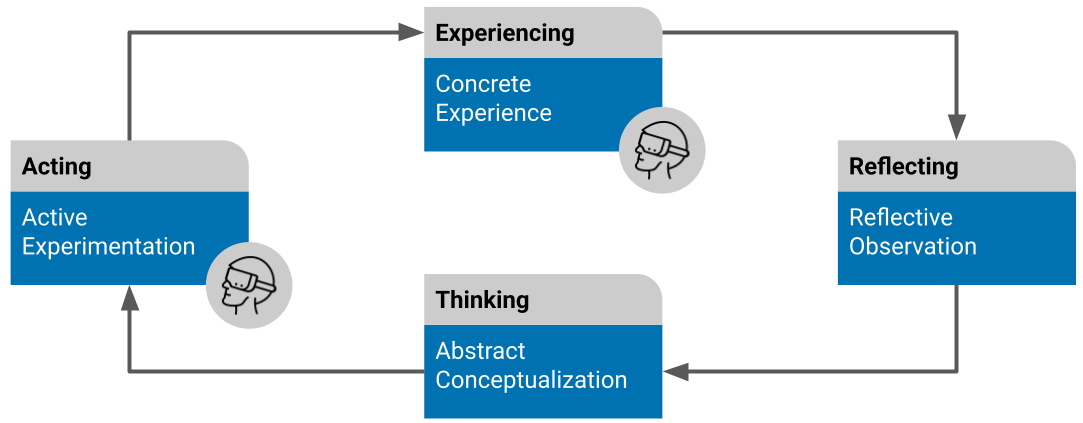
\includegraphics[width=0.9\linewidth]{pictures/ExperientialLearningCycle2.png}
	\captionsetup{labelfont=bf,textfont=it}
	\caption[The Experiential learning cycle as defined by Kolb \cite{kolb:1984:experiential}.]{The Experiential learning cycle as defined by Kolb \cite{kolb:1984:experiential}. Icons mark the stages where \acrshort{xr} could potentially be leveraged the most.\label{fig:learningCycle}}
\end{figure}

Computers can help to shift subjects we are not able to experience first hand (due to cost, risk, geographic distance, or the abstract nature of the topic) into an experiential learning scenario. That raises an important research question: \textbf{How can interactive applications beneficially be implemented in teaching?} We answer this question in \autoref{chap:ExGoer} by introducing a novel experiential learning framework. \Acrshort{xr} can increase this effect additionally due to its often spatial and haptic aspects.
The stages \emph{Concrete Experience} and \emph{Active Experimentation} are particularly suited to carry out in an \acrshort{xr} setting, because of their interactive nature. \acrshort{xr} can increase the interaction and immersion of those stages and therefore raise the impact of these experiences.
As a consequence, several research approaches in the current literature leverage \acrshort{xr} and its subcategories \acrshort{ar}, \acrshort{mr}, and \acrshort{vr} for experiential learning (e.g. \cite{asad2021virtual}, \cite{majgaard2020virtual}, \cite{wang2007experiential}, \cite{pueschel:2013:MRCG}). For experiential learning in application, see chapter \autoref{chap:ExGoer}.

\section{Skill Learning \label{sec:skill}}
Several research approaches suggest that the performance of a skill is superior when the context of skill application resembles the circumstances the skill was acquired in \cite{godden1975context}, \cite{ruitenberg2012context}, \cite{smith2001environmental}, \cite{anderson1998contextual}, \cite{wright1991contextual}. Therefore, it might be beneficial to create authentic learning scenarios through the means of \acrshort{mr}.

The haptic nature of skill learning --- motor skill learning in particular --- makes it not only a good fit for \acrshort{mr}, but also experiential learning. When approaching the subject of motor skill learning, a research question arises: \textbf{What is the state of the art for visualizing feedback for motor skill learning in \acrlong{mr}?} That question is being answered by a thorough literature survey in \autoref{chap:visualCueSurvey}. One of the most prevalent feedback methods we found in the literature were superimposed human avatars. As a consequence, a further research question emerged: \textbf{How can superimposed humanlike avatars be registered to facilitate motor skill learning?} This question will be answered in \autoref{chap:registration}.

Visualizing feedback for motor skill learning raises questions that have been answered in similar domains, but do not yield the same results here: \textbf{How can viewpoint selection take motion feedback into consideration?} In \autoref{chap:viewpoint}, we explore the literature regarding this question and propose a novel method to answer it. In conlusion, when considering feedback for motor skill learning in mixed reality, a final question emerges: \textbf{How can \acrlong{mr} systems be leveraged to support in-situ skill learning?} We answer this questions with a novel approach in \autoref{chap:omnipresent}.


Fitts and Posner introduced in 1967 a thee-stage model of skill learning (sometimes also called \emph{psychomotor learning}), categorizing the progress of an individual. More detail on the skill learning stages, especially in the context of physical activity, is provided in \autoref{sec:stages}.

\section{Situated Learning \label{sec:situated}}
Lave and Wenger introduced in 1991 the concept of \emph{Situated Learning}~\cite{lave:wenger:1991}. This theory concentrates on the acquisition of skills in the professional context. Lave and Wenger describe how learning often occurs in the form of apprenticeship (e.g. in professional sports or traditional crafts), where learning takes place in the same social and physical context where the skills are applied. Furthermore, they state that learning general rules does not necessarily carry over into specific scenarios. Therefore, it could be beneficial for the learning to take place in these circumstances~\cite[p. 34]{lave:wenger:1991}. This could be achieved by the use of \acrshort{mr}.